\documentclass[12pt]{article}


% -------------------- PAQUETES --------------------
\usepackage[utf8]{inputenc}
\usepackage[spanish]{babel}
\usepackage[margin=2.54cm]{geometry}
\usepackage{graphicx}
\usepackage{xcolor}
\usepackage{venndiagram}


% -------------------- CARGA DE ARCHIVOS EXTERNOS --------------------
% ----------------- UTILIDADES PARA DAR UN MEJOR FORMATO DE DOCUMENTO -----------------  


\definecolor{azul}{rgb}{0.0039, 0.3098, 0.6196}


% Formato para el indice general ...........
\makeatletter
    \renewcommand{\@dotsep}{1.5}
    \renewcommand{\l@section}{\@dottedtocline{1}{1.5em}{2.3em}}
    \renewcommand{\l@subsection}{\@dottedtocline{2}{3.8em}{3.2em}}
    \renewcommand{\l@subsubsection}{\@dottedtocline{3}{7.0em}{4.1em}}
\makeatother

% --------- COMANDOS PERSONALIZADOS PARA LA PORTADA DE LAS TAREAS, TRABAJOS Y PROYECTOS ---------

\newcommand{\rutaLogo}[1]{\newcommand{\RutaLogo}{#1}}
\newcommand{\tema}[1]{\newcommand{\Tema}{#1}}
\newcommand{\etiquetaAutores}[1]{\newcommand{\EtiquetaAutores}{#1}}
\newcommand{\alumno}[1]{\newcommand{\Alumno}{#1}}
\newcommand{\materia}[1]{\newcommand{\Materia}{#1}}
\newcommand{\docente}[1]{\newcommand{\Docente}{#1}}
\newcommand{\ciclo}[1]{\newcommand{\Ciclo}{#1}}
\newcommand{\fecha}[1]{\newcommand{\Fecha}{#1}}
\newcommand{\periodo}[1]{\newcommand{\Periodo}{#1}}



% -------------------- DEFINICIÓN DE LA PORTADA --------------------
\rutaLogo{../../../RecursosGlobales/Img/logo_tec_azuay.png}
\tema{\\ \vspace{1cm} Actividad N°2: \\Taller - Fin de la Unidad N°1 \\ \vspace{1.7cm}}
\etiquetaAutores{Alumno:}
\alumno{Eduardo Mendieta \vspace{1cm}}
\materia{Matemática \vspace{1cm}}
\docente{Lcda. Vilma Duchi \vspace{1cm}}
\ciclo{Primer Ciclo \vspace{1.1cm}}
\fecha{03 de junio de 2024 \vspace{1cm}}
\periodo{Abril 2024 - Agosto 2024}



% -------------------- INFORME --------------------
\begin{document}

    \begin{titlepage}

    \centering

    \includegraphics[width=0.11\textwidth]{\RutaLogo} 

    \vspace{0.3cm}
    \textcolor{azul}{\Large \textbf{Instituto Superior Universitario Tecnológico del Azuay \\}}
    \vspace{0.3cm}
    \textcolor{azul}{\Large \textbf{Tecnología Superior en Big Data}}
    
    % 1. ---------------- TEMA -------------------------
    
    {\Large\textbf{\Tema}}
    
    % 2. ---------------- AUTOR(ES) -------------------------
    \textcolor{azul}{\large \textbf{\EtiquetaAutores} \\}
    \vspace{0.3cm}
    {\large \Alumno}

    % 3. ---------------- MATERIA -------------------------
    \textcolor{azul}{\large \textbf{Materia:} \\}
    \vspace{0.3cm}
    {\large \Materia}


    % 3. ---------------- DOCENTE -------------------------
    \textcolor{azul}{\large \textbf{Docente:} \\}
    \vspace{0.3cm}
    {\large \Docente}


    % 3. ---------------- Ciclo -------------------------
    \textcolor{azul}{\large \textbf{Ciclo:} \\}
    \vspace{0.3cm}
    {\large \Ciclo}


    % 3. ---------------- FECHA -------------------------
    \textcolor{azul}{\large \textbf{Fecha:} \\}
    \vspace{0.3cm}
    {\large \Fecha}

    % 3. ---------------- PERIODO -------------------------
    \textcolor{azul}{\large \textbf{Periodo Académico:} \\}
    \vspace{0.3cm}
    {\large \Periodo}
 
\end{titlepage}

  
    \section*{\centering Actividades de fin de la Unidad N°1}

        % ACTIVIDAD 1 -------------------------------------------------------
        \subsection*{\textbf{\centering ACTIVIDAD 1}}

            \begin{enumerate}
                \item \textbf{Dados los siguientes conjuntos:}\par$A = \{x / x \in N\}$\\$B = \{ x \in N / x \geq 4 \}$\\$C = \{ x \in N / 2 < x > 7 \}$\\$D = \{ x \in R / -3 \leq x \geq 4 \}$\par\textbf{Exprese cada conjunto por tabulación y comprensión:} 
                    \begin{itemize}
                        \item \textbf{Tabulación}
                            \par$A = \{1, 2, 3, 4, 5, 6, 7, 8, 9, 10, ...\}$
                            \par$B = \{4, 5 ,6, 7, 8, 9, 10, 11, 12, ...\}$
                            \par$C = \{3, 4, 5, 6, 8, 9, 10, 11, 12, ...\}$
                            \par$D = \{-3, -2, -1, 0, 1, 2, 3, 4, ...\}$
                        \item \textbf{Comprensión}
                            \par$A = \{x / x \in N\}$
                            \par$B = \{x / x \in N, x > 3\}$
                            \par$C = \{x / x \in N, x > 2, x \neq 7\}$
                            \par$D = \{x / x \in R, x \geq -3\}$
                    \end{itemize}
                \item \textbf{Realice Diagramas de Venn del ejercicio anterior.}
                
            \end{enumerate}

            % ACTIVIDAD 2: ---------------------------------------------------------
            \subsection*{\textbf{\centering ACTIVIDAD 2}}

            \begin{enumerate}
                \item \textbf{De acuerdo a los elementos del diagrama de Ven realice las operaciones:}
                    \begin{figure}[!h]
                        \centering
                        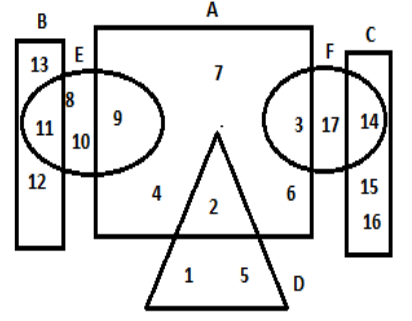
\includegraphics[width=0.5\textwidth]{Img/Tarea2/DiagVennActividad2.png}
                    \end{figure}

                    \begin{enumerate}
                        \item $A \cup B =$
                        \item $B \cap A =$
                        \item $A \cup C =$
                        \item $C \cap A =$
                        \item $A \cup D =$
                        \item $D \cap A =$
                        \item $C - F =$
                        \item $A - A =$
                        \item $D - A =$
                        \item $B^C - A^C =$
                        \item $C - A =$
                        \item $(E \cap B)^C = $
                    \end{enumerate}
            \end{enumerate}

        % ACTIVIDAD 3: -------------------------------------------------------------------
        \subsection*{\textbf{\centering ACTIVIDAD 3}}

            \begin{enumerate}
                \item \textbf{Resuelva los siguientes problemas:}
                    \begin{enumerate}
                        \item \textbf{Se dice que en la Ciudad de Cuenca 550 personas ven los canales D, E o F, 220 ven el canal D, 150 ven el canal E Y 100 no ven el canal F, los que ven por lo menos 2 canales son 120 ¿cuántos ven los tres canales?}
                        
                            \vspace{1cm}
                            \begin{venndiagram3sets}[labelA = D, labelB = E, labelC = F, labelABC = e, labelOnlyAB = b, labelOnlyAC = d, labelOnlyBC = f, labelOnlyA = a, labelOnlyB = c, labelOnlyC = g]
                                
                            \end{venndiagram3sets}

                            \begin{enumerate}
                                \item $Ec_1: U = a + b + c + d + e + f + g = 550\\Ec_2: D = a + b + d + e = 220\\Ec_3: E = b + c + e + f = 150\\Ec_4: (D \cup E) - F = a + b + c = 100\\Ec_5: (D \cap E) \cup (E \cap F) \cup (F \cap D) = b + d + e + f = 120$
                                \item Igualando $Ec_2$ con $Ec_4:\\220 - b - d - e = 100 - b - c\\- b - d - e + b + c = 100 - 220\\- d - e + c = - 120\\ - d = - 120 + e - c\\Ec_6: d = 120 - e + c$
                                \item Igualando $Ec_3$ con $Ec_5:\\150 - c - e - f = 120 - d - e - f\\- c - e - f + d + e + f = 120 - 150\\- c + d = - 30\\Ec_7: d = - 30 + c$
                                \item Igualando $Ec_6$ con $Ec_7:\\120 - e + c = - 30 + c\\- e + c - c = - 30 - 120\\- e = - 150\\e = 150$
                            \end{enumerate}
            
                            
                            \textbf{Respuesta:} El número de personas que ven los 3 canales es 150.

                        \item \textbf{De un grupo de estudiantes de entrenamiento deportivo: 19 practican básquet y natación, 37 practican solo natación, 30 practican básquet, Si 14 no practican ningún deporte de los mencionados. ¿Cuántos estudiantes hay en ese grupo?}
                    \end{enumerate}
            \end{enumerate}    

\end{document}